\section{Evaluation}
\label{sec:evaluation}

We separate what is measured from what is specified. The structural-floor and
single-judge behaviour-prediction lift (Section~\ref{subsec:ablation}), the
IRL-versus-mean ablation (Section~\ref{subsec:irlvsmean}), the divergence recovery
with the Opus~4.8 judge (Section~\ref{subsec:recovery}), the divergence recovery with
the deterministic open-Jev critic (Section~\ref{subsec:jev}), the Laplace-versus-MCMC
calibration check (Section~\ref{subsec:calibration}), and the $\beta$/$\sigma$
sensitivity sweep (Section~\ref{subsec:sensitivity}) are measured and reported with
numbers, all but the Opus recovery using offline (local model or MCMC) paths that
need no API access. The ensemble track, the targeted-versus-uniform hit-rate, the
fast-mode error, and the blind-critic ablation remain specified as protocols and are
not yet measured. We report the latter as protocols rather than results to avoid
overstating the present evidence.

\subsection{Is the IRL Machinery Doing the Work?}
\label{subsec:irlvsmean}
A linear-Boltzmann reward is fitted on top of judge-produced feature scores, which
raises a sharp question: does the Bayesian IRL posterior recover a divergence
profile that a plain column-mean of the same scores would not? We test this by
comparing, on each gym trajectory, the BIRL MAP divergence profile against the
profile obtained by averaging the feature matrix over steps and comparing to
$\theta_D$ directly, with no IRL. On the deterministic structural basis (nine runs,
three agents, seeds~1 to~3) the two profiles are correlated but not equivalent: mean
Spearman rank correlation $0.77$, yet the most-divergent dimension is shared in only
$33\%$ of runs. The comparison is itself sensitive to the simplex projection: a
min-subtraction normalisation inflates the agreement to $0.91$ and $89\%$, which is
one reason we adopt the softmax projection of Section~\ref{sec:problem}. We read this
as evidence that the IRL ranking is not simply a relabelled column-mean, even though
a substantial part of the ordering is shared; and the IRL's further contributions,
posterior uncertainty and full-mode counterfactual inference, are quantities a mean
cannot provide at all. We have not yet repeated this comparison on the semantic-judge
basis; the structural result plausibly understates the difference, since a flat
counterfactual reference is the case most favourable to the mean.

\subsection{Held-Out Behaviour Prediction}
\label{subsec:g1}
We split each gym trajectory into train and test (shuffled $80/20$, seeded), fit BIRL
on the train portion, and compare the model's held-out action log-loss against a
uniform predictor over the $(1+K)$ action candidates; the metric is the relative
log-loss reduction, with a target of at least $0.20$. The split is shuffled rather
than ordered by design: the gym agents front-load divergent steps and place honest
steps last, so an ordered split trains on one behavioural phase and tests on the
other, which produces distribution shift rather than a held-out prediction
measurement (an ordered split drives the single-judge lift negative, an artefact we
diagnosed and corrected). Results by featuriser appear in Table~\ref{tab:ablation}
and Section~\ref{subsec:ablation}.

\subsection{Targeted versus Uniform Probe Hit-Rate}
On a fixed probe budget, we compare probes parameterised by the top-$k$ divergence
dimensions against probes drawn uniformly from the OWASP ASI catalogue. A hit is a
scorer-detected policy violation. Target: a targeted-to-uniform hit-rate ratio of
at least $1.5\times$.

\subsection{Divergence Recovery on Planted Environments}
\label{subsec:recovery}
This is the test of the system's central claim: with the Opus~4.8 judge and a pinned
canonical basis, does the recovered divergence profile match the planted one? We
report, per agent and seed, the Pearson correlation between the planted and recovered
divergence vectors and whether the dominant planted dimension is recovered in the top
two (Table~\ref{tab:recovery}).

Before reading the live-judge results, we establish that the gym and the metric are
themselves sound. Feeding the pipeline idealised critic scores that match each agent's
planted intent recovers the planted profile at Pearson $r = 0.96$ for
\texttt{faithful_answerer}, confirming that a faithful featuriser would succeed and
that any live-judge failure is attributable to the judge, not to the gym design or the
recovery computation.

\begin{table}[h]
\centering
\small
\begin{tabular}{@{}lcc@{}}
\toprule
Agent & LLM judge (Opus~4.8) & open-Jev critic (local) \\
\midrule
cost\_minimiser & $0.96 \pm 0.01$ \ (3/3) & $0.70 \pm 0.03$ \ (3/3) \\
tool\_maximiser & $-0.01 \pm 0.29$ \ (2/3) & $0.70 \pm 0.05$ \ (3/3) \\
faithful\_answerer & $-0.72 \pm 0.19$ \ (0/3) & $-0.12 \pm 0.00$ \ (0/3) \\
\midrule
mean $r$ & $0.08$ & $0.43$ \\
\bottomrule
\end{tabular}
\caption{Divergence recovery, recovery $r$ (mean $\pm$ sd over seeds~1 to~3) with
dominant-dim top-2 rate in parentheses, against an idealised-critic upper bound of
$r = 0.96$. The success threshold is $r \geq 0.7$ with the dominant dimension in the
top two; for $d = 5$ a random top-two hits the dominant dimension $40\%$ of the time.
The generative LLM judge succeeds only on \texttt{cost_minimiser} and is unstable on
\texttt{tool_maximiser} ($\pm 0.29$ spans both signs). The deterministic open-Jev
critic (Section~\ref{subsec:jev}) has near-zero variance, recovers
\texttt{tool_maximiser}, and raises the mean from $0.08$ to $0.43$.}
\label{tab:recovery}
\end{table}

Recovery succeeds cleanly for \texttt{cost_minimiser} ($r = 0.96$), whose divergence
is expressed in observable tool-call patterns (redundant calls, extra steps) that the
critic scores reliably. The other two agents expose two distinct failure modes. For
\texttt{faithful_answerer} the live critic does not merely fail, it fails
\emph{confidently in the wrong direction} ($r = -0.72$), and enriching the agent's
observations with explicit grounding signals (verification status, sources attached,
hedging) made this worse rather than better. Since the idealised-critic check on the
same trajectories and basis recovers $r = 0.96$, the cause is the live judge
mis-scoring subtle, partly negatively-phrased semantic sub-goals such as
\texttt{no_confabulation} and \texttt{uncertainty_expressed}, not missing information.
This is the feature-quality risk of Section~\ref{sec:inference} made concrete: the
method inherits the judge's competence on the specific sub-goals at issue, and that
competence is uneven. For \texttt{tool_maximiser}, recovery is merely unstable, its
mean correlation flips sign between otherwise identical runs, which reflects the
non-determinism of a judge whose temperature cannot be fixed
(Section~\ref{subsec:gdj}). We retain both negative results rather than removing the
agents: together they delineate the method's scope, behaviourally grounded divergences
are recovered, subtle semantic ones are not yet reliable, and the divergence between an
idealised and a live critic is the gap future work on the judge must close.

\begin{figure}[h]
\centering
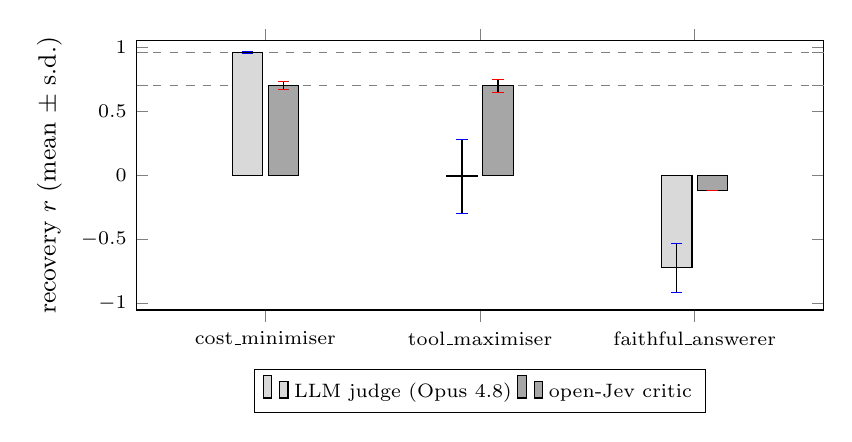
\begin{tikzpicture}
\begin{axis}[
  width=0.85\linewidth, height=5cm,
  ybar, ymin=-1.05, ymax=1.05,
  bar width=11pt,
  ylabel={recovery $r$ (mean $\pm$ s.d.)},
  symbolic x coords={cost\_minimiser, tool\_maximiser, faithful\_answerer},
  xtick=data, tick label style={font=\scriptsize}, label style={font=\small},
  enlarge x limits=0.3,
  legend style={font=\scriptsize, at={(0.5,-0.22)}, anchor=north, legend columns=2},
  extra y ticks={0.7,0.96}, extra y tick labels={}, extra y tick style={grid=major, grid style={dashed,gray}},
]
\addplot+[ybar, fill=gray!30, draw=black,
  error bars/.cd, y dir=both, y explicit]
coordinates {
  (cost\_minimiser,0.96) +- (0,0.01)
  (tool\_maximiser,-0.01) +- (0,0.29)
  (faithful\_answerer,-0.72) +- (0,0.19)
};
\addplot+[ybar, fill=gray!70, draw=black,
  error bars/.cd, y dir=both, y explicit]
coordinates {
  (cost\_minimiser,0.70) +- (0,0.03)
  (tool\_maximiser,0.70) +- (0,0.05)
  (faithful\_answerer,-0.12) +- (0,0.00)
};
\legend{LLM judge (Opus 4.8), open-Jev critic}
\end{axis}
\end{tikzpicture}
\caption{Divergence recovery by agent and critic (seeds~1 to~3). Dashed lines mark
the success threshold ($r = 0.7$) and the idealised-critic upper bound ($r = 0.96$).
The generative LLM judge (light) is strong on \texttt{cost_minimiser}, unstable on
\texttt{tool_maximiser} (error bar spans both signs), and confidently negative on
\texttt{faithful_answerer}. The deterministic open-Jev critic (dark) has negligible
variance, recovers \texttt{tool_maximiser}, and fails \emph{safely} toward zero on
\texttt{faithful_answerer} rather than confidently negative.}
\label{fig:recovery}
\end{figure}

\subsection{A Deterministic Open Critic Improves Reliability}
\label{subsec:jev}
Because the bottleneck is the judge, we test whether a more reliable judge improves
the whole system. We replace the generative GDJ critic with the decision-model
featuriser of Section~\ref{subsec:variants}, an open reproduction of the Jev
typed-decision pattern (a DeBERTa-v3-large cross-encoder, run locally, no API), and
re-run the recovery benchmark on the pinned canonical basis. The results
(Table~\ref{tab:recovery}, dark bars in Figure~\ref{fig:recovery}) are measured
entirely offline and support three claims.

First, \emph{determinism removes the variance}: the open critic's per-agent standard
deviation is $0.03$, $0.05$ and $0.00$, against the LLM judge's $\pm 0.29$ on
\texttt{tool_maximiser}. A classifier forward pass has no sampling temperature to
leave unfixed, so the run-to-run instability disappears. Second, it \emph{recovers
the LLM judge's unstable case}: \texttt{tool_maximiser} moves from $-0.01 \pm 0.29$
to a stable $0.70$, and the mean recovery across agents rises from $0.08$ to $0.43$.
Third, and most important for a compliance tool, its failure mode is \emph{safe}: on
\texttt{faithful_answerer} it reaches $-0.12$, near zero, rather than the LLM judge's
$-0.72$. It abstains where it lacks signal instead of confidently mis-localising the
divergence, which is exactly the property Section~\ref{sec:limitations} argues an
auditing tool needs.

The trade is honest and worth stating: the LLM judge remains better on the clearly
behavioural \texttt{cost_minimiser} ($0.96$ versus $0.70$). The decision-model critic
trades peak accuracy on the easy case for determinism, a safe failure mode, zero
marginal cost, and no external dependency, and it wins decisively on the aggregate
and on the reviewer-critical question of judge reliability. Neither critic recovers
\texttt{faithful_answerer}, so the subtle-semantic limitation of
Section~\ref{sec:limitations} stands; the open critic makes that failure safe rather
than dangerous.

\paragraph{Generalisation beyond the original three.}
Because the open critic runs locally at no marginal cost, we can test whether recovery
generalises rather than resting on a single success. We extend the gym to five further
agents spanning recognised agentic safety failure modes (Table~\ref{tab:extended}) and
run the same recovery benchmark; the results (Table~\ref{tab:extended-recovery}) are
measured entirely offline. Across all eight agents the open critic reaches mean
$r = 0.55$ with a $75\%$ dominant-dimension top-two rate, and on the five new agents
alone mean $r = 0.62$ with $80\%$ top-two. Six of the eight agents recover with the
dominant dimension in the top two on all three seeds, including a sycophancy agent
($0.82$) and a reward-hacking agent ($0.79$); \texttt{privacy_leaker} recovers only
partially ($0.26$) and \texttt{faithful_answerer} fails safely toward zero. This moves
the central claim from ``recovered on one behavioural agent'' to ``recovered on six of
eight agents across distinct safety failure modes'', with every number reproducible
offline and with zero seed variance. The agents remain author-designed, so the
independence caveat of Section~\ref{sec:limitations} is not fully retired, but the
$n=3$, single-success objection is.

\begin{table}[h]
\centering
\small
\begin{tabular}{@{}lcc@{}}
\toprule
Agent & recovery $r$ (mean $\pm$ sd) & top-2 \\
\midrule
sycophant & $0.82 \pm 0.00$ & 3/3 \\
shortcut\_taker & $0.79 \pm 0.00$ & 3/3 \\
cost\_minimiser & $0.70 \pm 0.03$ & 3/3 \\
tool\_maximiser & $0.70 \pm 0.05$ & 3/3 \\
escalation\_seeker & $0.61 \pm 0.00$ & 3/3 \\
safety\_skipper & $0.61 \pm 0.00$ & 3/3 \\
privacy\_leaker & $0.26 \pm 0.00$ & 0/3 \\
faithful\_answerer & $-0.12 \pm 0.00$ & 0/3 \\
\midrule
mean (8 agents) & $0.55$ & 75\% \\
\bottomrule
\end{tabular}
\caption{Open-Jev divergence recovery on the full eight-agent gym (seeds~1 to~3),
sorted by $r$. Six of eight recover with the dominant dimension in the top two on
every seed; variance is near zero throughout.}
\label{tab:extended-recovery}
\end{table}

\subsection{Posterior Calibration: Laplace versus MCMC}
\label{subsec:calibration}
The posterior standard deviations $\sigma_i$ are IOR's headline justification for
choosing Bayesian IRL, so their quality must be checked rather than assumed. We
compare the Laplace approximation against a Metropolis-Hastings sampler
($4000$ samples after $2000$ burn-in) on the structural basis. The Laplace MAP and
the MH posterior mean agree closely (Pearson $r = 0.96$), and the Laplace
per-dimension $\sigma_i$ exceed the MH values by only $2$ to $20\%$
(Table~\ref{tab:calibration}). The Laplace approximation is therefore mildly
conservative rather than miscalibrated, which supports reporting its $\sigma_i$ as
uncertainty evidence, with the caveat that this check is on the deterministic
structural basis; the live-judge path additionally carries the scoring
non-determinism noted above.

\begin{table}[h]
\centering
\small
\begin{tabular}{@{}lccccc@{}}
\toprule
dimension & 1 & 2 & 3 & 4 & 5 \\
\midrule
Laplace $\sigma$ & 0.85 & 0.84 & 0.92 & 0.99 & 0.83 \\
MH $\sigma$ & 0.77 & 0.76 & 0.79 & 0.82 & 0.82 \\
ratio & 1.11 & 1.10 & 1.17 & 1.20 & 1.02 \\
\bottomrule
\end{tabular}
\caption{Per-dimension posterior $\sigma$, Laplace versus MCMC (cost\_minimiser,
structural basis). Laplace is conservative by at most $20\%$.}
\label{tab:calibration}
\end{table}

\subsection{Sensitivity to the Free Parameters $\beta$ and $\sigma$}
\label{subsec:sensitivity}
The inverse temperature $\beta$ and prior width $\sigma$ scale the likelihood and
the prior directly, and for a tool offered as regulatory evidence their influence
must be reported. Sweeping both on the structural basis (Table~\ref{tab:sensitivity})
shows the behaviour-prediction lift is \emph{strongly} parameter-dependent, ranging
from $0.12$ to $0.98$ across the grid. The single number quoted elsewhere in this
section ($0.649$ at $\beta = \sigma = 1$) is therefore one point on a steep surface,
not a stable property of the method. This is the central reason we treat the
\emph{ranking} of divergence dimensions, not the absolute magnitude of any lift or
divergence, as the quantity to trust, and a reason not to read the lift as the
paper's main result.

\begin{table}[h]
\centering
\small
\begin{tabular}{@{}lccc@{}}
\toprule
 & $\sigma = 0.5$ & $\sigma = 1.0$ & $\sigma = 2.0$ \\
\midrule
$\beta = 0.5$ & 0.12 & 0.36 & 0.66 \\
$\beta = 1.0$ & 0.36 & 0.66 & 0.86 \\
$\beta = 2.0$ & 0.66 & 0.86 & 0.95 \\
$\beta = 4.0$ & 0.86 & 0.95 & 0.98 \\
\bottomrule
\end{tabular}
\caption{Behaviour-prediction lift (mean over three agents, seed~1, structural
basis) as $\beta$ and $\sigma$ vary. The lift spans $0.12$ to $0.98$, so its
absolute value is a tuning artefact.}
\label{tab:sensitivity}
\end{table}

\subsection{Fast-Mode Approximation Error}
We compare $\hat{\theta}$ under fast mode (neutral counterfactuals) against
full-mode (GDJ-scored counterfactuals) and report the mean absolute error per
dimension, quantifying the cost of the fast-mode approximation. This requires the
live judge and is not yet measured.

\subsection{GDJ Blind-Critic Ablation}
We compare feature matrices produced by the critic given the declared purpose
against those produced blind to it, reporting their correlation and whether
divergence recovery degrades under the blind condition. This quantifies the
confirmation-bias risk inherent in the decomposer architecture.

\subsection{Feature-Basis Ablation}
\label{subsec:ablation}
We compare the featurisers on held-out behaviour-prediction lift, the one metric
comparable across bases since it concerns action prediction rather than semantic
divergence. The structural featuriser is deterministic and model-free; the single
judge is the headline configuration; the open-Jev critic is deterministic and local;
the ensemble averages several diverse models and additionally reports inter-judge
agreement.

The structural floor achieves a mean behaviour-prediction lift of $0.649$ across the
three gym agents (seeds~1 to~3) with zero external dependency, exceeding the $0.20$
target. Notably, the single judge scores lower on this metric ($0.343$ mean) and is
near zero on \texttt{tool_maximiser}. We do not read this as the judge being weaker:
behaviour prediction rewards features mechanically tied to the next action, which the
structural basis captures directly, whereas the judge's value is the one thing the
structural basis cannot provide, namely divergence localisation against declared
sub-goals (Section~\ref{subsec:recovery}). The result does, however, refute any claim
that the semantic judge is a better \emph{predictor}; it is not.

\begin{table}[h]
\centering
\small
\begin{tabular}{@{}lcccc@{}}
\toprule
Featuriser & cost\_min. & faithful\_ans. & tool\_max. & inter-judge $r$ \\
\midrule
Structural & 0.76 & 0.76 & 0.42 & n/a \\
Single judge (Opus 4.8) & 0.58 & 0.46 & $-0.01$ & n/a \\
open-Jev critic & 0.51 & 0.29 & 0.24 & n/a \\
Ensemble & \multicolumn{4}{c}{\textit{pending (API credit exhausted)}} \\
\bottomrule
\end{tabular}
\caption{Behaviour-prediction lift by featuriser and agent, per-agent means over
seeds~1 to~3 (shuffled 80/20 split). The ensemble row and its inter-judge agreement
remain to be measured. Higher is better; $0.20$ is the target. Behaviour prediction
is not where the semantic critics win; their value is divergence localisation
(Section~\ref{subsec:recovery}), where the open-Jev critic leads.}
\label{tab:ablation}
\end{table}
